%\newtheorem{The}{Théorème}
%\newtheorem{Pro}[The]{Proposition}
%\newtheorem{Pre}[The]{Preuve}
%\newtheorem{Def}[The]{Définition}
%\newtheorem{Exemp}[The]{Exemple}
%%%%%%%%%%%%%%%%%%%%%%%%%%%%%%%%%%%%%%%%%%%%
%%%%%%%%%%%%%%%%%%%%%%%%%%%%%%%%%%%%%%%%%%%%
%%%%%%%%%%%%%%%%%%%%%%%%%%%%%%%%%%%%%%%%%%%%
%\begin{Exemp}[....]\end{Exemp}
%\begin{The}[Pythogore] 
%La somme des carrés des longueurs côtés adjacents à l'angle droit d'un triangle rectangle est égale au carré de la longueur de l'hypothénuse de ce triangle. \end{The} 
%%%%%%%%%%%%%%%%%%%%%%%%%%%%%%%%%%%%%%%%%%%%
%%%%%%%%%%%%%%%%%%%%%%%%%%%%%%%%%%%%%%%%%%%%
%%%%%%%%%%%%%%%%%%%%%%%%%%%%%%%%%%%%%%%%%%%%
%%%%%%%%%%%%%%%%%%%%%%%%%%%%%%%%%%%%%%%%%%%%
%%%%%%%%%%%%%%%%%%%%%%%%%%%%%%%%%%%%%%%%%%%%
% web.univ-ubs.fr/lmam/gouno/BAYES/COURS/Cours1.pdf
% web.univ-ubs.fr/lmam/gouno/BAYES/COURS/Cours2.pdf
% web.univ-ubs.fr/lmam/gouno/BAYES/COURS/Cours3.pdf
% web.univ-ubs.fr/lmam/gouno/BAYES/COURS/Cours4.pdf
% web.univ-ubs.fr/lmam/gouno/BAYES/COURS/Cours5.pdf
% web.univ-ubs.fr/lmam/gouno/BAYES/COURS/Cours6.pdf
%%%%%%%%%%%%%%%%%%%%%%%%%%%%%%%%%%%%%%%%%%%%
%%%%%%%%%%%%%%%%%%%%%%%%%%%%%%%%%%%%%%%%%%%%
%%%%%%%%%%%%%%%%%%%%%%%%%%%%%%%%%%%%%%%%%%%%
%%%%%%%%%%%%%%%%%%%%%%%%%%%%%%%%%%%%%%%%%%%%
%%%%%%%%%%%%%%%%%%%%%%%%%%%%%%%%%%%%%%%%%%%%


\section{Estimateur de Bayes}
Comme nous l’avons déjà fait remarquer, la prise d’une décision, ici le choix d’un estimateur, va engendrer un coût que l’on va quantifier à l’aide de la fonction de perte. En pratique, on cherche une décision qui minimise en moyenne la fonction de coût.
\begin{Def}
On appelle estimateur de Bayes associé à un coût $L$ et à une distribution a priori $\pi$, toute décision $\delta^{\pi}}$ qui minimise le risque de Bayes $r(\pi, \delta)$.\newline
On a :
$$\delta^{\pi}(x)=\underset{\delta \in \mathcal{D}}{\arg\min}\textrm{ } r(\pi,\delta)$$
\end{Def}
Remarquons que d’après la proposition précédente (Risque de Bayes $r(\pi,\delta)$), une estimateur peut également être défini comme étant une décision qui minimise la moyenne suivant la prédictive f(x) du coût a posteriori.
\subsection*{Fonctions de coût usuelles}
\subsubsection*{Coût quadratique}
\begin{Def}
La fonction de coût quadratique est la fonction définie par :
$$L(\theta,\delta(x))=(\theta-\delta(x))^{2}$$
Une variante de cette fonction de coût est une fonction de coût quadratique pondérée de la forme :
$$L(\theta,\delta(x))=w(\theta)(\theta-\delta(x))^{2}$$
\end{Def}
\begin{Pro}
Sous l’hypothèse d’un coût quadratique, l’estimateur de Bayes $\delta^{\pi}}(x)$ de $\theta$ associé à la loi a priori $\pi$ est la moyenne a posteriori de $\theta$ :
$$\delta^{\pi}(x)=\mathbb{E}^{(.|\pi)}(\theta)=\int_{\theta\in\Theta}L(\theta,\delta(x))\pi(\theta|x)\textrm{d}\theta$$
\end{Pro}
\begin{Pre}
Par définition, l’estimateur de Bayes minimise le coût a posteriori \textit{i.e.}
$$\rho(\pi,\delta)=\mathbb{E}^{\pi(.|x)}[L(\theta,\delta(x))]$$
Sous l’hypothèse d’un coût quadratique, on a :
$$\rho(\pi,\delta)=\mathbb{E}^{\pi(.|x)}[L(\theta,\delta(x))] = \mathbb{E}^{\pi(.|x)}(\theta^{2})-2\delta(x)\mathbb{E}^{\pi(.|x)}(\theta)+\delta^{2}(x)$$
Il s’agit d’un polynôme du second degré en $\delta(x)$. Il sera minimum en $\mathbb{E}^{\pi(.|x)}(\theta)$.
\end{Pre}
\begin{Exemp}
\begin{enumerate}
  \item 
\end{enumerate}

\end{Exemp}







    

  \item[] \textit{}.
  \item[] \textit{}.
  \item[] \textit{}.


  
 
    
    

% web.univ-ubs.fr/lmam/gouno/BAYES/COURS/Cours1.pdf
% web.univ-ubs.fr/lmam/gouno/BAYES/COURS/Cours2.pdf
% web.univ-ubs.fr/lmam/gouno/BAYES/COURS/Cours3.pdf
% web.univ-ubs.fr/lmam/gouno/BAYES/COURS/Cours4.pdf
% web.univ-ubs.fr/lmam/gouno/BAYES/COURS/Cours5.pdf
% web.univ-ubs.fr/lmam/gouno/BAYES/COURS/Cours6.pdf



\begin{figure}[H]\begin{center}\includegraphics[scale=1]{ilu/probab .png}\end{center}\end{figure}


\begin{lstlisting}[language=html]
  
\end{lstlisting}


%% La dernière image est probab28




%




%%%%%%%%%%%%%%%%%%%%%%%%%%%%%%%%%%%%%%%%%%%%%%%%%%%%%%%%%%%%%%%%%%%%%%%%%%
%%%%%%%%%%%%%%%%%%%%%%%%%%%%%%%%%%%%%%%%%%%%%%%%%%%%%%%%%%%%%%%%%%%%%%%%%%%%%%%%%%%%%%%%%%%%%%%%%%%%%%%%%%%%%%%
%%%%%%%%%%%%%%%%%%%%%%%%%%%%%%%%%%%%%%%%%%%%%%%%%%%%%%%%%%%%%%%%%%%%%%%%%%%%%%%%%%%%%%%%%%%%%%%%%%%%%%%%%%%%%%%
%%%%%%%%%%%%%%%%%%%%%%%%%%%%%%%%%%%%%%%%%%%%%%%%%%%%%%%%%%%%%%%%%%%%%%%%%%%%%%%%%%%%%%%%%%%%%%%%%%%%%%%%%%%%%%%%%%%%%%%%%%%%%%%%%%%%%%%%%%%%%%%%%%%%%%%%%%%%%%%%%%%%%%%%%%%%%%%%%%%%%%%%%
%%%%%%%%%%%%%%%%%%%%%%%%%%%%%%%%%%%%%%%%%%%%%%%%%%%%%%%%%%%%%%%%%%%%%%%%%%%%%%%%%%%%%%%%%%%%%%%%%%%%%%%%%%%
%%%%%%%%%%%%%%%%%%%%%%%%%%%%%%%%%%%%%
%%%%%%%%%%%%%%%%%%%%%%%%%%%%%%%%%%%%%%%%%%%%%%%%%%%%%%%%%%%%%%%%%%%%%%%%%%%%%%%%%%%%%%%%%%%%%%%%%%%%%%%%%%%%%%%%%%%%%%%%%%%%%%%%%%%%%%%%%%%%%%%%%%%%%%%%%%%%%%%%%%%%%%%%%%%%%%%%%%%%%%%%%%%%%%%%%%%%%%%%%%%%%%%%%%%%%%%%%%%%%%%%%%%%%%%%%%%%%%%%%%%%%%%%%%%%%%%%%%%%%%%%%%%%%%%%%%%%%%%%%%%%%%%%%%%%%%%%%%%%%%%%%%%%%%%%%%%%%%%%%%%%%%%%%%%%%
%%%%%%%%%%%%%%%%%%%%%%%%%%%%%%%%%%%%%
%%%%%%%%%%%%%%%%%%%%%%%%%%%%%%%%%%%%%
%%%%%%%%%%%%%%%%%%%%%%%%%%%%%%%%%%%%%
%%%%%%%%%%%%%%%%%%%%%%%%%%%%%%%%%%%%%






%%%%%%%%%%%%%%%%%%%%%%%%%%%%%%%%%%%%%
%%%%%%%%%%%%%%%%%%%%%%%%%%%%%%%%%%%%%%%%%%%%%%%%%%%%%%%%%%%%%%%%%%%%%%%%%%
%%%%%%%%%%%%%%%%%%%%%%%%%%%%%%%%%%%%%%%%%%%%%%%%%%%%%%%%%%%%%%%%%%%%%%%%%%
%%%%%%%%%%%%%%%%%%%%%%%%%%%%%%%%%%%%%%%%%%%%%%%%%%%%%%%%%%%%%%%%%%%%%%%%%%
%%%%%%%%%%%%%%%%%%%%%%%%%%%%%%%%%%%%%

\begin{figure}[H]\begin{center}\includegraphics[scale=1]{ilu/adeq .png}\end{center}\end{figure}



Soit $X$ la \textit{var} égale au numéro affiché par le dé après un lancer. Par l'énoncé, on observe la valeur de $X$ sur chacun des $n$ individus (dés) d'un échantillon avec $n = 100$ : $(x_{1}; \dots ; x_{n})$ (avec $x_{i} \in \{1; \dots ; 6\})$. On forme alors un vecteur des effectifs $(n_{1}; n_{2}; \dots ; n_{6}) = (18; 23; \dots ; 15)$.\newline
Dire que le dé n'est pas truqué signifie que $X$ suit la loi uniforme $\mathit{U}(\{1; \dots ; 6\})$ :
$$\mathbb{P}(X=i) = \frac{1}{6}, \textrm{ } i \in \{1,\dots, 6\}$$
La problématique est la suivante : \textit{est-ce que les données nous permettent d'affirmer que X ne suit pas la loi $\mathit{U}(\{1; \dots ; 6\})$} ?\newline
\\
Ainsi, pour une analyse graphique, on propose les commandes :
\begin{lstlisting}[language=html]
> nb = c(18, 23, 19, 12, 11, 15)
> bar = barplot(nb / 100, col = "white")
> points(bar, rep(1 / 6, 6), type = "h",col="red")
\end{lstlisting}
\begin{figure}[H]\begin{center}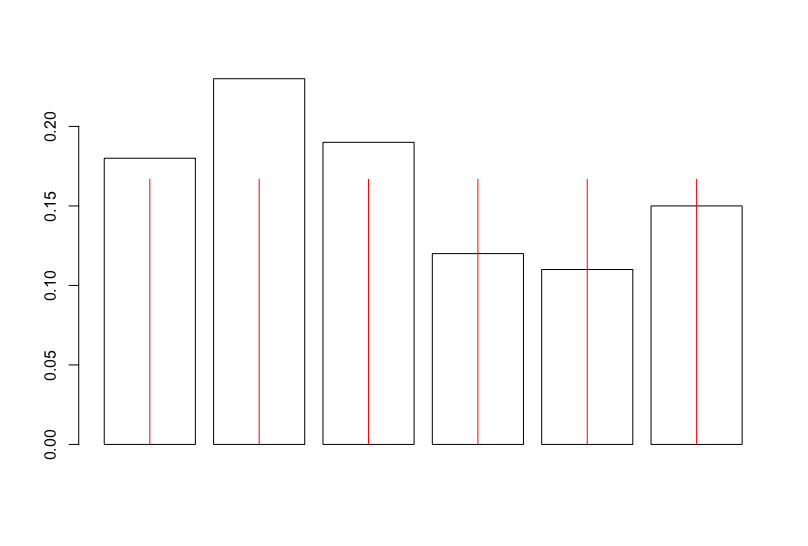
\includegraphics[scale=1]{ilu/adeq14.png}\end{center}\end{figure}
Il est difficile de conclure au vu des différences observées.\newline
On peut utiliser le test du Chi-deux d'adéquation à une loi pour y voir plus clair. On considère alors les hypothèses :
\begin{itemize}
  \item $H_{0}$ : "X suit la loi uniforme $\mathit{U}(\{1; \dots ; 6\})$"
  \item $H_{1}$ : "X ne suit pas la loi uniforme $\mathit{U}(\{1; \dots ; 6\})$".
\end{itemize}
Les valeurs sont regroupées en $k = 6$ classes : $C_{1} = \{1\}$, $C_{2} = \{2\}$,\dots, $C_{6} = \{6\}$.\newline
On considère les commandes :
\begin{lstlisting}[language=html]
> nb
[1] 18 23 19 12 11 15
> proba = rep(1 / 6, 6)
> chisq.test(nb, p = proba)$p.value
[1] 0.2757299
\end{lstlisting}
Notons qu'aucun "Warning message" n'apparaît ; les conditions d'application du test sont vérifiées.\newline
Comme $p$-valeur $> 0,05$, les données ne nous permettent pas de rejeter $H_{0}$. Ainsi, on ne peut pas affirmer que le dé est truqué.

%%%%%%%%%%%%%%%%%%%%%%%%%%%%%%%%%%%%%

%%%%%%%%%%%%%%%%%%%%%%%%%%%%%%%%%%%%%

On indique dans le tableau suivant le nombre de fois qu'un chiffre apparaît dans les $608$ premières décimales de $\pi$ : 
\begin{center}
\begin{tabular}{|c|c|c|c|c|c|c|c|c|c|c|}
\hline
\textbf{Chiffre}        & 0  & 1  & 2  & 3  & 4  & 5  & 6  & 7  & 8  & 9  \\ \hline
\textbf{Nombre de fois} & 60 & 62 & 67 & 68 & 64 & 56 & 62 & 44 & 58 & 67 \\ \hline
\end{tabular}
\end{center}
\textit{Peut-on affirmer, au risque $5\%$, que les décimales ne sont pas équiréparties ?}

%%%%%%%%%%%%%%%%%%%%%%%%%%%%%%%%%%%%%

%%%%%%%%%%%%%%%%%%%%%%%%%%%%%%%%%%%%%

Soit $X$ la var égale au chiffre affiché par une décimale (que l'on suppose donc aléatoire).\newline
Par l'énoncé, on observe la valeur de $X$ sur chacun des n individus (décimales) d'un échantillon avec $n = 608$ : $(x_{1}; \dots ; x_{n})$ (avec $x_{i} \in \{0; \dots ; 9 \})$. On forme alors un vecteur des effectifs $(n_{1}; n_{2}; \dots ; n_{10}) = (60; 62; : : : ; 67)$. Dire que les décimales sont équiréparties signifie que $X$ suit la loi uniforme $\mathit{U}(\{0; \dots ; 9\})$ :
$$\mathbb{P}(X=i) = \frac{1}{10}, \textrm{ } i \in \{1,\dots, 9\}$$

La problématique est la suivante : \textit{est-ce que les données nous permettent d'affirmer que X ne suit pas la loi $\mathit{U}(\{0; \dots ; 9\})$} ?\newline
\\
\begin{itemize}
  \item $H_{0}$ : "X suit la loi uniforme $\mathit{U}(\{1; \dots ; 9\})$"
  \item $H_{1}$ : "X ne suit pas la loi uniforme $\mathit{U}(\{1; \dots ; 9\})$".
\end{itemize}
On peut utiliser le test du Chi-deux d'adéquation à une loi. Les valeurs sont regroupées en k = 10
classes : $C_{1} = \{0\}$, $C_{2} = \{1\}$,\dots, $C_{10} = \{9\}$.\newline
On considère les commandes :
\begin{lstlisting}[language=html]
> nb = c(60, 62, 67, 68, 64, 56, 62, 44, 58, 67)
> proba = rep(1 / 10, 10)
> chisq.test(nb, p = proba)$p.value
[1] 0.585888
\end{lstlisting}
Notons qu'aucun "Warning message" n'apparaît ; les conditions d'application du test sont vérifiées.\newline
Comme $p$-valeur $> 0,05$, les données ne nous permettent pas de rejeter $H_{0}$. Ainsi, au risque $5\%$, on ne peut pas affirmer que le décimales de $\pi$ soient équiréparties.

%%%%%%%%%%%%%%%%%%%%%%%%%%%%%%%%%%%%%%%%%%%%%
%%%%%%%%%%%%%%%%%%%%%%%%%%%%%%%%%%%%%%%%%%%%%
%%%%%%%%%%%%%%%%%%%%%%%%%%%%%%%%%%%%%%%%%%%%%
%%%%%%%%%%%%%%%%%%%%%%%%%%%%%%%%%%%%%%%%%%%%%
%%%%%%%%%%%%%%%%%%%%%%%%%%%%%%%%%%%%%%%%%%%%%
%%%%%%%%%%%%%%%%%%%%%%%%%%%%%%%%%%%%%%%%%%%%%
%%%%%%%%%%%%%%%%%%%%%%%%%%%%%%%%%%%%%%%%%%%%%
%%%%%%%%%%%%%%%%%%%%%%%%%%%%%%%%%%%%%%%%%%%%%
%%%%%%%%%%%%%%%%%%%%%%%%%%%%%%%%%%%%%%%%%%%%%
%%%%%%%%%%%%%%%%%%%%%%%%%%%%%%%%%%%%%%%%%%%%%

Lindström, spécialiste de la génétique et de l'hybridation du maïs, a croisé deux types récessifs de maïs : le type vert-zébré et le type doré. Si les lois de la génétique sont respectées obtient :
\begin{itemize}
  \item  "vert" avec la probabilité $9/16$
  \item  "doré" avec la probabilité $3/16$
  \item  "vert-zébré" avec la probabilité $3/16$
  \item  "doré-vert-zébré" avec la probabilité $1/16$
\end{itemize}
On effectue $1301$ croisements. On obtient les résultats suivants :
\begin{center}
\begin{tabular}{|c|c|c|c|c|}
\hline
\textbf{Type}          & "vert" & "doré" & "vert-zébré" & "doré-vert-zébré" \\ \hline
\textbf{Nombre defois} & 773    & 231     & 238            & 59                   \\ \hline
\end{tabular}
\end{center}
\textit{Peut-on dire que les lois de la génétique ne sont pas respectées ?} (on fera une analyse graphique convenable, puis un test statistique adapté au risque $5\%$).

\varepsilon

%%%%%%%%%%%%%%%%%%%%%%%%%%%%%%%%%%%%%%%%%%%%%
%%%%%%%%%%%%%%%%%%%%%%%%%%%%%%%%%%%%%%%%%%%%%
%%%%%%%%%%%%%%%%%%%%%%%%%%%%%%%%%%%%%%%%%%%%%
%%%%%%%%%%%%%%%%%%%%%%%%%%%%%%%%%%%%%%%%%%%%%
%%%%%%%%%%%%%%%%%%%%%%%%%%%%%%%%%%%%%%%%%%%%%
%%%%%%%%%%%%%%%%%%%%%%%%%%%%%%%%%%%%%%%%%%%%%
%%%%%%%%%%%%%%%%%%%%%%%%%%%%%%%%%%%%%%%%%%%%%
%%%%%%%%%%%%%%%%%%%%%%%%%%%%%%%%%%%%%%%%%%%%%
%%%%%%%%%%%%%%%%%%%%%%%%%%%%%%%%%%%%%%%%%%%%%
%%%%%%%%%%%%%%%%%%%%%%%%%%%%%%%%%%%%%%%%%%%%%













\begin{figure}[H]\begin{center}\includegraphics[scale=1]{ilu/norm .png}\end{center}\end{figure}